%!TEX root = ../rapport.tex

\chapter{Planning}
Le déroulement aura un penchant Agile. A savoir qu'au lieu de faire les grosses phases "Analyse, conception, réalisation", nous opterons plutôt pour des cycles itératifs. C'est-à-dire que nous commencerons petit, en pure environnement de test, où nous mettrons en place une qualité de service. Lorsque ceci est prêt, nous passerons à une échelle plus proche de la production et ajouterons d'autres services et ainsi de suite. Il sera ainsi possible de rapidement se rendre compte de ce qui pourrait poser problème par la pratique et de corriger le tir plus facilement.

\begin{figure}[H]
    \begin{center}
        \centering 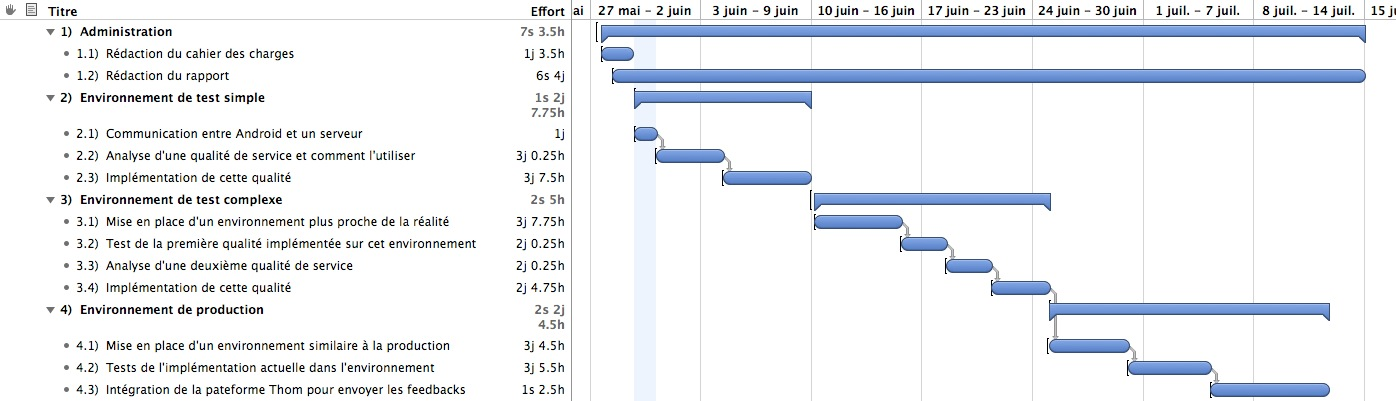
\includegraphics[width=1.5\linewidth, angle=90]{CDC/planning_bachelor_v1}
    \end{center}
\end{figure}
% section structure_du_document (end)